\scanpage{98}
% archive sheet number: 97
% source lines 01-02; multiplication arcs above and below the factors
\figure{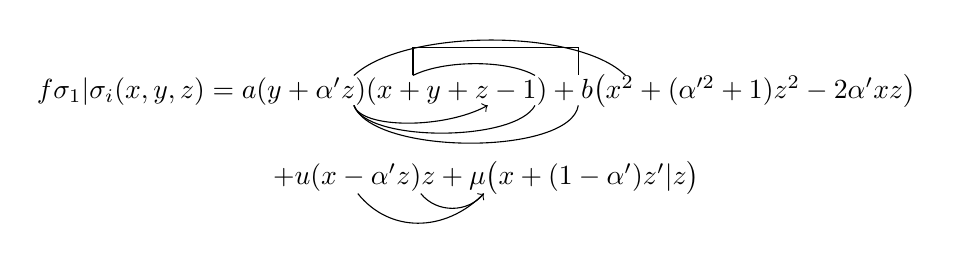
\begin{tikzpicture}[x=1cm,y=1cm]
\node[anchor=west] at (0,0) {$f\unsure{\sigma_1|\sigma_i}(x,y,z)=a(y+\alpha'z)(x+y+z-1)+b\bigl(x^2+(\alpha^{\prime 2}+1)z^2-2\alpha'xz\bigr)$};
\node[anchor=west] at (3,-1.1) {$+u(x-\alpha'z)z+\mu\bigl(x+(1-\alpha')\unsure{z'|z}\bigr)$};
\draw (4.15,.2) .. controls (4.8,.8) and (7.0,.8) .. (7.6,.2);
\draw (4.9,.2) -- (4.9,.55) -- (7.0,.55) -- (7.0,.2);
\draw (4.9,.2) .. controls (5.3,.4) and (6.1,.4) .. (6.45,.2);
\draw[->] (4.15,-.18) .. controls (4.25,-.48) and (5.3,-.48) .. (5.85,-.18);
\draw (4.15,-.18) .. controls (4.3,-.65) and (6.2,-.65) .. (6.45,-.18);
\draw (4.15,-.18) .. controls (4.4,-.82) and (6.9,-.82) .. (7.0,-.18);
\draw[->] (4.2,-1.3) .. controls (4.6,-1.8) and (5.3,-1.8) .. (5.8,-1.3);
\draw (5.0,-1.3) .. controls (5.2,-1.55) and (5.6,-1.55) .. (5.8,-1.3);
\end{tikzpicture}}
% source lines 03-05
\[
\begin{aligned}
={}&bx^2+ay^2+\bigl(a\alpha'+b(1+\alpha^{\prime 2})\inserted{\unsure{+|-}u\alpha'}\bigr)z^2\\
&+(-a\alpha)yz+(a\alpha'-2b\alpha'+u)zx+\deleted{\unsure{2}}axy\\
&+\mu x+(-a)y+\bigl(-a\alpha'+\mu(1-\alpha')\bigr)z
\end{aligned}
\]
% source line 06
\[
\deleted{\unsure{a=}}\boxed{b=a}
\]
% source lines 07-08
\[
\begin{aligned}
&a\alpha'+b(1+\alpha^{\prime 2})\unsure{-|+}u\alpha'=b\\
\text{i.e.}\quad&a\bigl(\underbrace{\alpha^{\prime 2}+\alpha'+1\deleted{\unsure{+\alpha-1|-1}}}_{\unsure{1.|10|1|0}}\bigr)=u\alpha'
\qquad\text{i.e.}\quad\boxed{u=-\alpha a}
\end{aligned}
\]
% source lines 09-14
\[
\begin{aligned}
-a\alpha&=u\qquad\text{ok}\\
a\alpha'-2b\alpha'+u&=a\quad\text{i.e.}\quad
\unsure{a}(\unsure{a\alpha'|\alpha'|4\alpha'}-2\alpha'+\underbrace{\deleted{\unsure{\alpha'}}\inserted{-\alpha}-1}_{\alpha'})=0\quad\text{ok}\\
a&=a\qquad\text{ok}\\
\boxed{\mu=-a}&\\
-a&=\mu\quad\text{ok}\\
-a\alpha'+\mu(\deleted{1}-\alpha')&=\deleted{\mu}\quad\text{i.e.}\quad
\deleted{\unsure{+a(-\alpha'-a\alpha')}}\inserted{-\alpha'(a+\mu)=0}\quad\text{ok}
\end{aligned}
\]
% source line 15
\[
f(x,y,z)=a\unsure{q|\rho}(x,y,z)
\]
% source lines 16-17
\[
\boxed{\begin{aligned}
q(x,y,z)&=x(x+y+z-1)+(y^2+z^2)\unsure{-|+}\alpha yz-(y+z)\\
&=x^2+y^2+z^2-\alpha yz+zx+xy-(x+y+z)
\end{aligned}}\tag*{(19)}
\]
% source lines 18-21
Les fonctions quadr. \unsure{invariantes} sont donc celles de la forme $aq(x,y,z)+d$, celles qui sont nulles sur $S$ sont celles de la forme $aq(x,y,z)$.
